\documentclass[11pt]{article}
\usepackage[margin=2.5cm]{geometry}
\usepackage{amsmath,amssymb,amsthm}
\usepackage{array}
\usepackage{graphicx}
\usepackage[section]{placeins}
\usepackage{tikz}
\usetikzlibrary{arrows.meta,calc,decorations.pathreplacing}
\definecolor{conceptone}{RGB}{42,120,214}
\definecolor{concepttwo}{RGB}{235,104,52}

\newtheorem{definition}{Definition}
\newtheorem{requirement}{Requirement}
\newtheorem{proposition}{Proposition}
\theoremstyle{remark}
\newtheorem*{remark}{Remark}

\DeclareMathOperator{\softplus}{softplus}
\DeclareMathOperator{\vol}{vol}
\DeclareMathOperator{\softmax}{softmax}
\DeclareMathOperator{\BCE}{BCE}
\newcommand{\R}{\mathbb{R}}
\newcommand{\T}{\mathcal{T}}

\newenvironment{symbols}
  {\par\smallskip\noindent\small\begin{tabular}{@{}>{$}l<{$}@{\quad}p{0.82\linewidth}@{}}}
  {\end{tabular}\par\medskip}

\title{Story space: salient concepts as volumes in a story-conditioned latent space}
\date{}

\begin{document}
\maketitle

\section{Problem}

\begin{definition}[Story, paragraphs]
A story $s \in \T$ is a string of text from the space of texts $\T$. It is split into paragraphs $p_1, \dots, p_N \in \T$.
\end{definition}
\begin{symbols}
s & the story, a string of text \\
\T & the space of all strings of text \\
p_i & the story's $i$-th paragraph \\
N & the number of paragraphs in the story \\
\end{symbols}

\begin{definition}[Salient concept]
A salient concept $c \in \T$ is a string of text naming an idea the story contains. It need not be copied out of the story: the idea may never be mentioned directly. A story comes with a set of salient concepts $C_s = \{c_1, \dots, c_K\}$.
\end{definition}
\begin{symbols}
c & a salient concept, a string of text naming an idea \\
C_s & the set of the story's salient concepts \\
K & the number of salient concepts \\
\end{symbols}

\begin{definition}[Story state]
A story state $\sigma$ is a structured description of a moment of the story (characters, location, event, action). A fixed template $\tau$ renders it as text, $\tau(\sigma) \in \T$.
\end{definition}
\begin{symbols}
\sigma & a story state: characters, location, event, action \\
\tau & the fixed template that writes a state out as text \\
\tau(\sigma) & the text of state $\sigma$ \\
\end{symbols}

\begin{definition}[Story space]
The story space $\mathcal{Z}_s \subseteq \R^d$ is the latent space of story $s$. Every salient concept $c$ is a volume $B_c \subset \mathcal{Z}_s$ and every story state $\sigma$ is a point $z(\sigma) \in \mathcal{Z}_s$. A state is related to a concept when its point lies inside the concept's volume. Two concepts are related when their volumes overlap.
\end{definition}
\begin{symbols}
\mathcal{Z}_s & the story space of story $s$ \\
d & the number of dimensions of the story space \\
\R^d & the space of vectors of $d$ real numbers \\
B_c & the volume of concept $c$ in the story space \\
z(\sigma) & the point of state $\sigma$ in the story space \\
\end{symbols}

\begin{figure}[ht]
\centering
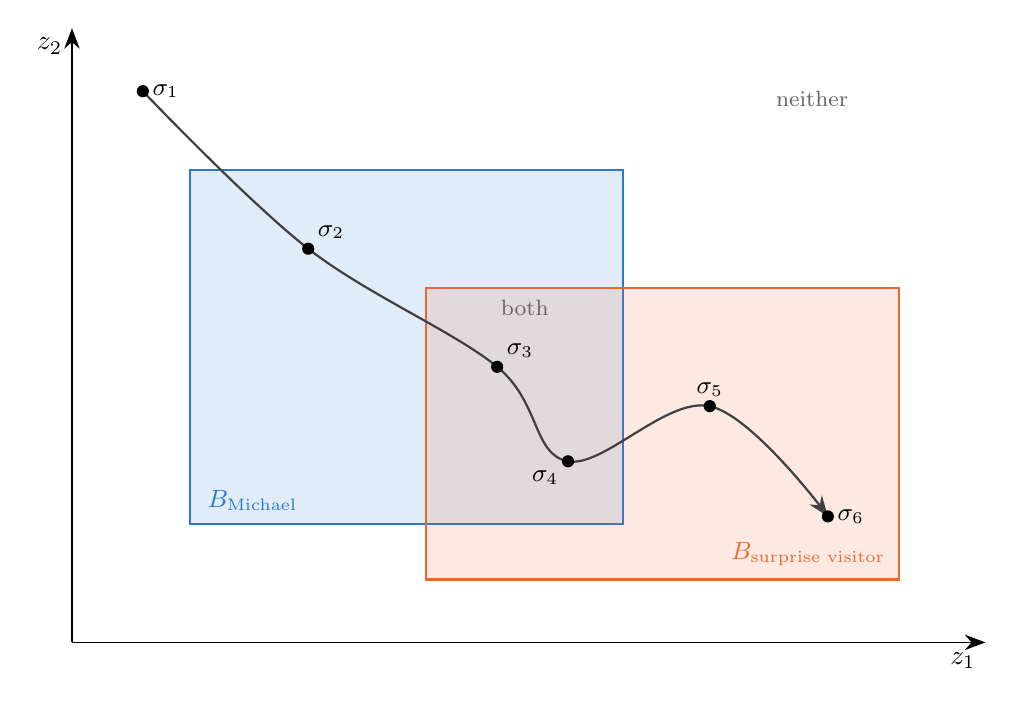
\begin{tikzpicture}[x=1cm, y=1cm, >={Stealth[length=2.6mm]}]
  \draw[->] (0,0) -- (11.6,0) node[below left] {$z_1$};
  \draw[->] (0,0) -- (0,7.8) node[below left] {$z_2$};

  \fill[conceptone, opacity=0.14] (1.5,1.5) rectangle (7.0,6.0);
  \draw[conceptone, thick] (1.5,1.5) rectangle (7.0,6.0);
  \fill[concepttwo, opacity=0.14] (4.5,0.8) rectangle (10.5,4.5);
  \draw[concepttwo, thick] (4.5,0.8) rectangle (10.5,4.5);

  \node[conceptone, anchor=south west, font=\small] at (1.6,1.55) {$B_{\text{Michael}}$};
  \node[concepttwo, anchor=south east, font=\small] at (10.45,0.85) {$B_{\text{surprise visitor}}$};
  \node[font=\footnotesize, text=black!60] at (5.75,4.25) {both};
  \node[font=\footnotesize, text=black!60] at (9.4,6.9) {neither};

  \draw[->, thick, black!75] plot[smooth, tension=0.6] coordinates
    {(0.9,7.0) (3.0,5.0) (5.4,3.5) (6.3,2.3) (8.1,3.0) (9.6,1.6)};

  \foreach \x/\y/\k/\pos in {0.9/7.0/1/right, 3.0/5.0/2/above right, 5.4/3.5/3/above right, 6.3/2.3/4/below left, 8.1/3.0/5/above, 9.6/1.6/6/right} {
    \fill[black] (\x,\y) circle (2.2pt);
    \node[\pos, font=\small] at (\x,\y) {$\sigma_{\k}$};
  }
\end{tikzpicture}
\caption{Illustration, not computed from data. Two concept volumes in a story space and the trajectory of SCENE\_1's states in story order. $z_1$ and $z_2$ are two of the story space's $d$ dimensions; $\sigma_k$ marks the point of the story's $k$-th state. $\sigma_1$, a warm sunny day, lies in neither volume. $\sigma_2$, Michael and Sarah setting out for a walk, lies only in $B_{\text{Michael}}$. $\sigma_3$, an unexpected knock at their door, and $\sigma_4$, Michael going down to check, lie in the overlap. $\sigma_5$, Sarah calling ``Who is it?'', and $\sigma_6$, no answer coming, lie only in $B_{\text{surprise visitor}}$.}
\label{fig:story-space}
\end{figure}

Figure~\ref{fig:story-space} shows two overlapping concept volumes and a story moving through them.

The story space is a conditioning of the general latent space of all texts: of all the places a text can occupy in the general space, the story picks out the region that it, its concepts and its states occupy.

\paragraph{Tasks.}
\begin{enumerate}
  \item[(T1)] Define the story space for $s$, given $s$ and $C_s$: the operation \texttt{encode\_basis}.
  \item[(T2)] Map a story state into the story space: the operation \texttt{encode\_from\_state}. States are described with arbitrary text, yet two states described with the same words must land on the same point.
  \item[(T3)] Find the boundaries of the volumes of the salient concepts.
\end{enumerate}

\paragraph{Requirements.}
\begin{requirement}[Non-degenerate volume]\label{req:volume}
The volume of a concept has non-zero width along every dimension of $\mathcal{Z}_s$.
\end{requirement}
\begin{requirement}[Containment]\label{req:contain}
A state related to concept $c$ maps to a point inside $B_c$. A state unrelated to $c$ maps outside it.
\end{requirement}
\begin{requirement}[Multiple membership]\label{req:multi}
A state may be related to several concepts at once, so volumes may overlap and a point may lie in several of them.
\end{requirement}
\begin{requirement}[Identity]\label{req:identity}
Equal states map to the same point: $\sigma = \sigma' \Rightarrow z(\sigma) = z(\sigma')$.
\end{requirement}
\begin{requirement}[Separation]\label{req:separation}
Different states map to different points: $\sigma \neq \sigma' \Rightarrow z(\sigma) \neq z(\sigma')$.
\end{requirement}
\begin{symbols}
\sigma' & a second story state, compared with $\sigma$ \\
\end{symbols}

\section{How Qwen encodes a text}\label{sec:qwen}

Qwen is used as it is: frozen, nothing in it trained. The figures were measured with Qwen3-8B, which has $L = 36$ layers and a latent space of $D = 4096$ dimensions.

\paragraph{A point in latent space.} Qwen splits a text $t$ into tokens $k = 0, \dots, n-1$. After each layer $\ell$ it holds, for every token, a point $h_{\ell,k}(t)$ in its latent space $\R^D$; $\ell = 0$ is the token's lookup before any layer.

\paragraph{The latent space.} $\R^D$ is a real vector space with the dot product $u \cdot v = \sum_{i=1}^{D} u_i v_i$, which gives lengths, angles and distances. All layers share it. The points are not normalised, and their lengths are bounded: the longest here is about $12{,}000$. The points crowd into a narrow cone whose apex is the space's zero, because training gives every point one large common component.

\paragraph{One point per token.} Qwen gives one point per token, not one per text. Each point summarises the text up to and including its token. The text ``Bob'' gives one point after each layer; a passage of $n$ tokens gives $n$.

\paragraph{A token's path through the layers.} Following one token from layer $0$ to layer $L$ gives a trajectory of $L+1$ points. Each step is one layer: the layer analyses the point, attending to the points of the tokens before it and passing the result through a feed-forward network, and adds what it finds to the point:
\begin{equation}
h_{\ell,k}(t) = h_{\ell-1,k}(t) + \Delta_{\ell,k}(t) .
\end{equation}

\paragraph{Where the information is.} In each point itself: in where it lies along the space's feature directions, not in how the points relate to each other.

\paragraph{Token $0$.} From layer $7$ on, the first token's point becomes an attention sink: about $185$ times longer than the others and the same for every text, whatever its first word. It is left out of everything below.

\begin{symbols}
t & any text given to Qwen \\
k & a token's position in the text, starting at $0$ \\
n & the number of tokens in the text \\
\ell & a layer of Qwen; $0$ means the lookup before the first layer \\
L & the number of Qwen's layers \\
D & the number of dimensions of Qwen's latent space \\
\R^D & Qwen's latent space \\
h_{\ell,k}(t) & the point in $\R^D$ that Qwen holds for token $k$ of text $t$ after layer $\ell$ \\
u, v & any two points of $\R^D$ \\
u_i & the $i$-th of the $D$ coordinates of $u$ \\
u \cdot v & the dot product of $u$ and $v$ \\
\Delta_{\ell,k}(t) & what layer $\ell$ adds to token $k$'s point \\
\end{symbols}

\subsection{Extending a text}

Three texts share a beginning:
\begin{center}
\begin{tabular}{@{}ll@{}}
A & ``Bob buys Alice coffee'' \\
A + B & ``Bob buys Alice coffee, because he loves her'' \\
A + C & ``Bob buys Alice coffee and bagels with salmon'' \\
\end{tabular}
\end{center}
B adds Bob's motivation; C adds a detail that changes nothing important. Figure~\ref{fig:abc} shows their points after layer $16$.

\begin{figure}[ht]
\centering
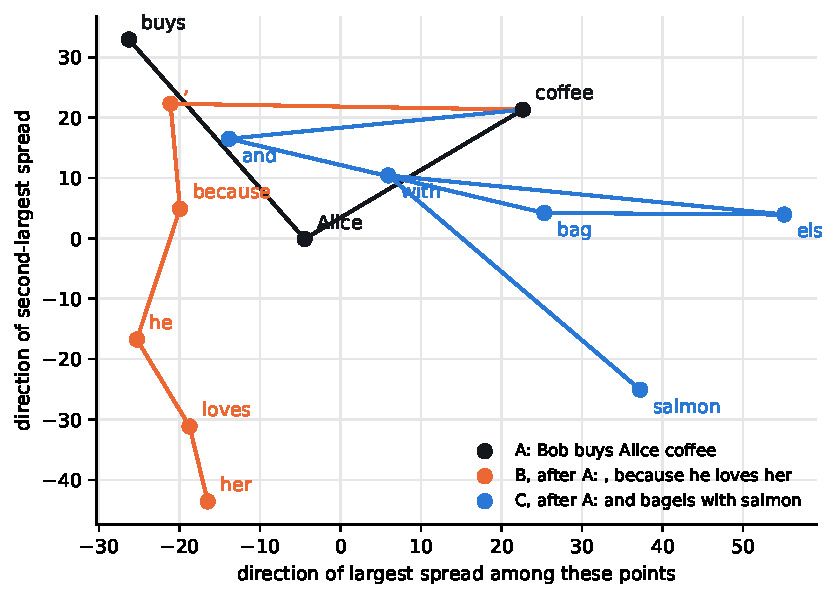
\includegraphics[width=0.85\linewidth]{figures/abc_points_layer16.pdf}
\caption{The points of A, A + B and A + C after layer $16$, token $0$ (``Bob'') left out. Black: A's points, shared by all three texts. Orange: the points B adds after A. Blue: the points C adds after A. Lines join the points in reading order. The $13$ points live in $\R^{4096}$; they are drawn along the two directions in which they differ most, which hold $34\%$ of their spread.}
\label{fig:abc}
\end{figure}

\paragraph{Salient information.} Write $I(t)$ for the salient information a text $t$ carries, and $V(t)$ for the volume that surrounds text $t$. We take as given:
\begin{equation}
\begin{gathered}
|V(A)| \approx |V(B)|, \qquad |V(A)| > |V(C)|, \\
|V(A + B)| \gg |V(A + C)|, \qquad |V(A)| \approx |V(A + C)| .
\end{gathered}
\end{equation}
What remains to be found is how Qwen encodes and represents this information.
\begin{symbols}
I(t) & the salient information text $t$ carries \\
V(t) & the volume that surrounds text $t$ \\
|V(t)| & the size of that volume \\
\end{symbols}

\paragraph{Shannon information.} The Shannon information of a text under Qwen is the number of bits Qwen needs to predict it, token by token:
\begin{equation}
H(t) = -\sum_{k} \log_2 p\bigl(\text{token}_k \mid \text{tokens before it}\bigr), \qquad H(B \mid A) = H(A + B) - H(A) .
\end{equation}
\begin{symbols}
H(t) & the Shannon information of text $t$ under Qwen, in bits \\
p(\text{token}_k \mid \cdot) & the probability Qwen gives token $k$ after reading the tokens before it \\
H(B \mid A) & the bits B costs once A has been read \\
\end{symbols}
Every token is scored, the first one included, by starting each text with Qwen's document separator.

\begin{table}[ht]
\centering
\begin{tabular}{@{}lr@{}}
text & $H$ (bits) \\
\hline
A & 63.4 \\
B & 50.8 \\
C & 72.6 \\
A + B & 92.1 \\
A + C & 111.9 \\
B, after A: $H(B \mid A)$ & 28.7 \\
C, after A: $H(C \mid A)$ & 48.6 \\
\end{tabular}
\caption{The Shannon information of every text under Qwen3-8B.}
\label{tab:shannon}
\end{table}


\begin{table}[ht]
\centering
\setlength{\tabcolsep}{4pt}
\begin{tabular}{@{}lll@{}}
salient information & Shannon information & holds \\
\hline
$|V(A)| \approx |V(B)|$ & $H(A) = 63.4$, $H(B) = 50.8$ & no: A costs a quarter more \\
$|V(A)| > |V(C)|$ & $H(A) = 63.4$, $H(C) = 72.6$ & no: C costs more \\
$|V(A + B)| \gg |V(A + C)|$ & $H(A + B) = 92.1$, $H(A + C) = 111.9$ & no: the reverse \\
$|V(A)| \approx |V(A + C)|$ & $H(A) = 63.4$, $H(A + C) = 111.9$ & no: A + C costs $76\%$ more \\
\end{tabular}
\caption{The relations of salient information, tested with Shannon information.}
\label{tab:relations}
\end{table}

None of the four relations holds for Shannon information (Tables~\ref{tab:shannon} to~\ref{tab:relations}). Every added token costs bits, so a longer text always carries more, and what costs most is what surprises Qwen: ``salmon'' costs $16.4$ bits, ``her'' in ``because he loves her'' $0.4$. Salient information is therefore not what Qwen's surprise measures.

\subsection{Properties of the function that measures salient information}\label{sec:properties}

The data give the function $I$ three properties:
\begin{enumerate}
  \item \textbf{It is not surprise.} Shannon information breaks all four relations (Table~\ref{tab:relations}), so the function cannot be built from Qwen's token probabilities.
  \item \textbf{It is not additive over tokens.} $|V(A)| \approx |V(A + C)|$ although A + C has five more tokens than A, so the function must give C's points almost nothing while giving B's a lot.
  \item \textbf{It is not distance.} B and C move the points by about the same amount: after layer $16$, the last points of A + B and A + C lie equally far from A's last point (cosine $0.34$ and $0.37$, distance $96$ and $95$). They move them in different directions (Figure~\ref{fig:abc}), so the function must tell directions apart.
\end{enumerate}
Together: the function is a projection onto a subspace of Qwen's latent space that keeps the directions B's points move in and discards the directions C's points move in.

\subsection{Movement}\label{sec:movement}

Figure~\ref{fig:abc-areas} shows the points of A, B and C as areas with their centroids after layers $1$, $10$, $20$ and $36$.

\begin{figure}[ht]
\centering
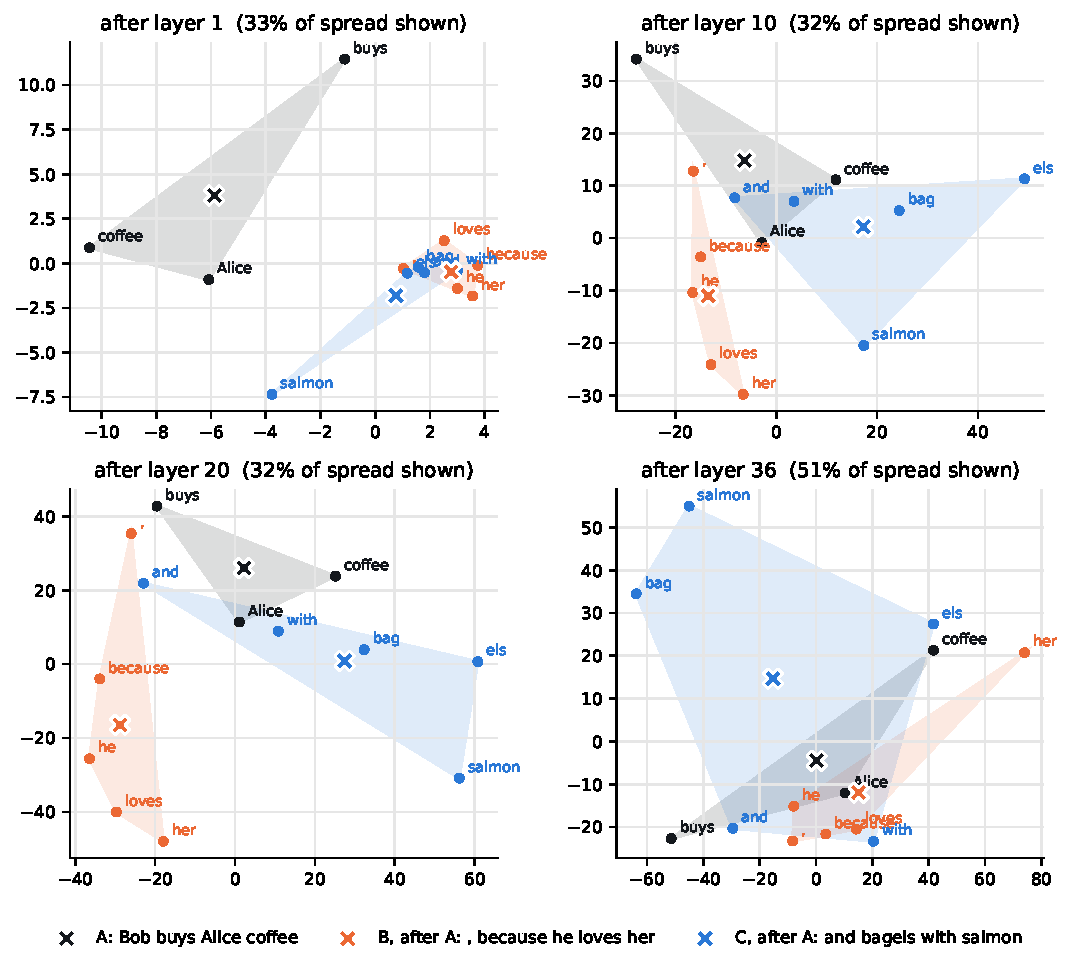
\includegraphics[width=\linewidth]{figures/abc_areas_by_layer.pdf}
\caption{The points of A, A + B and A + C after layers $1$, $10$, $20$ and $36$, token $0$ (``Bob'') left out. Black: A's points. Orange: the points B adds after A. Blue: the points C adds after A. Each shaded area is the smallest polygon around one colour's points; the cross is their centroid. Each panel draws its layer's $13$ points along the two directions in which they differ most, with the share of their spread those directions hold in the title.}
\label{fig:abc-areas}
\end{figure}

Figure~\ref{fig:separate-areas} runs A, B, C, A + B and A + C through Qwen separately and draws the area of each.

\begin{figure}[ht]
\centering
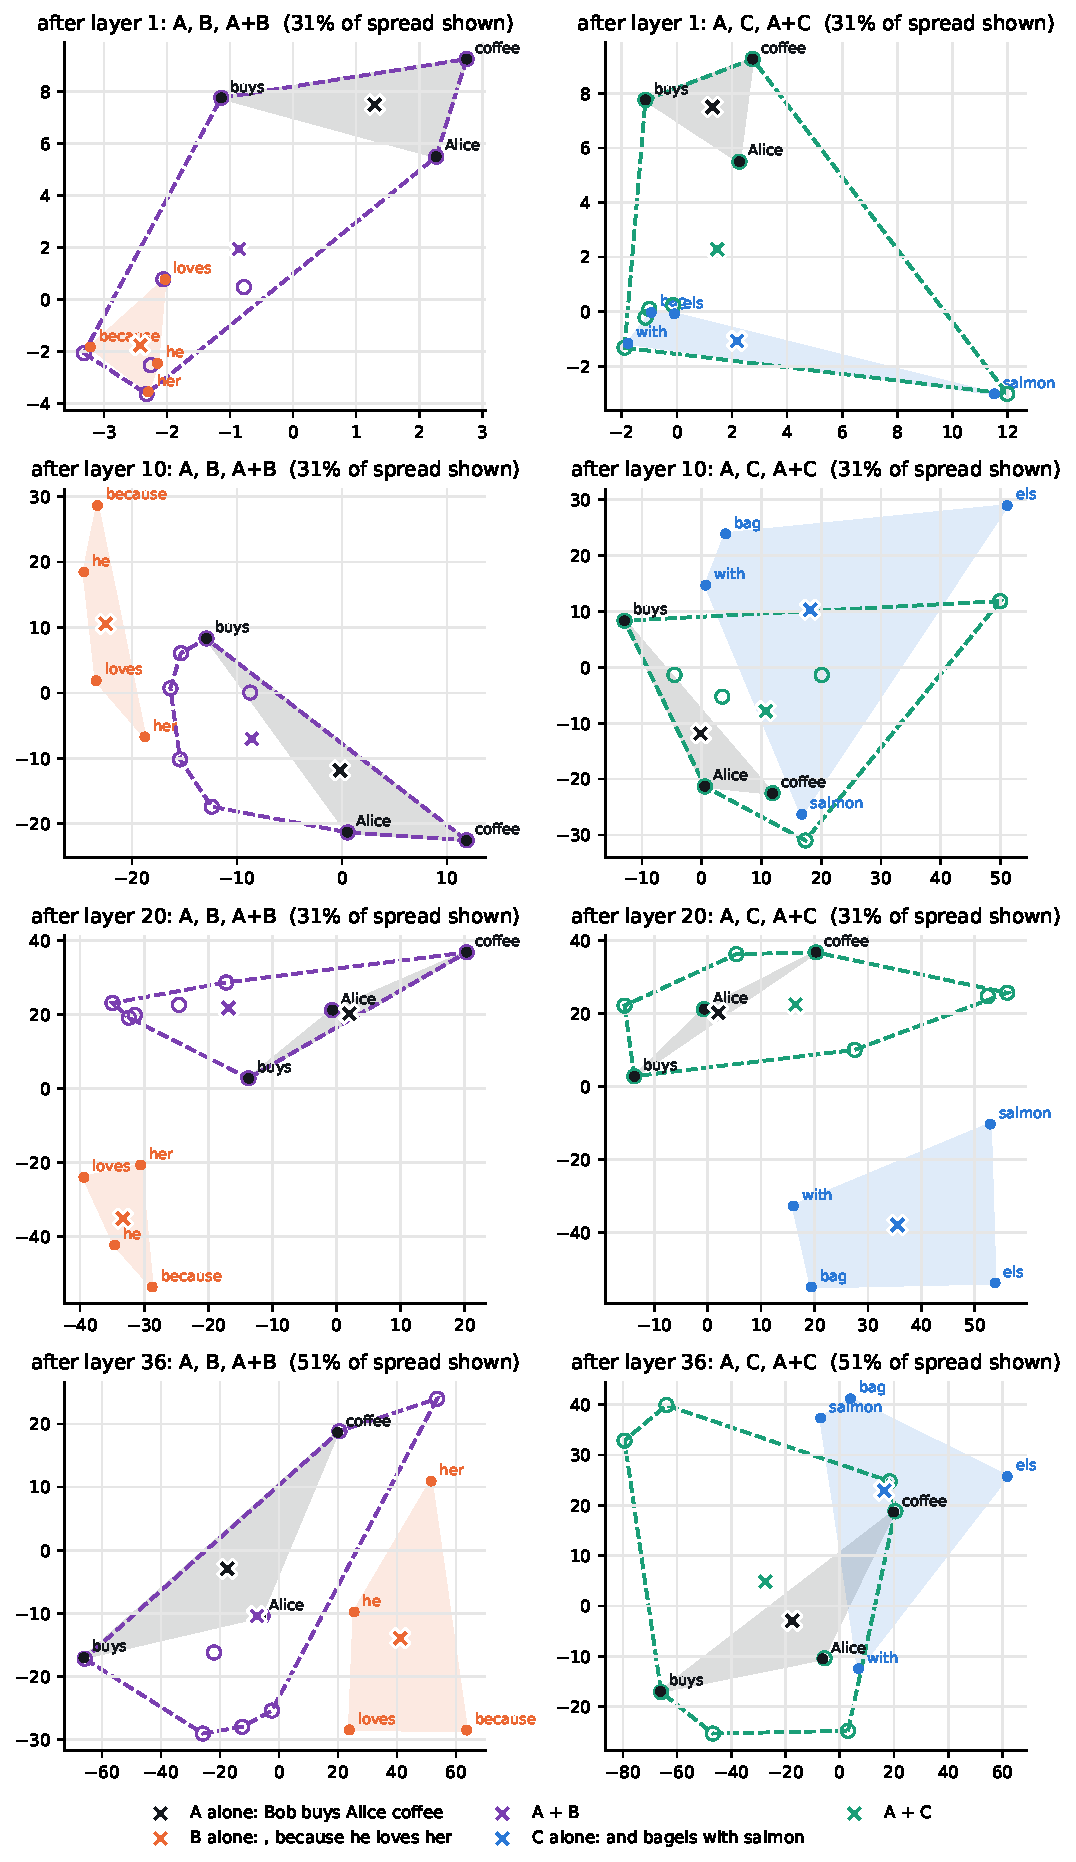
\includegraphics[width=\linewidth,height=0.8\textheight,keepaspectratio]{figures/separate_areas_by_layer.pdf}
\caption{A, B, C, A + B and A + C, each run through Qwen on its own, after layers $1$, $10$, $20$ and $36$, every text's token $0$ left out. Filled areas: A, B and C alone. Dashed outlines and hollow circles: A + B (left) and A + C (right). Crosses: centroids. Both panels of a row are drawn along the same two directions, those in which that layer's points differ most.}
\label{fig:separate-areas}
\end{figure}

Adding B or C never moves A's points: inside A + B and A + C they stay within $2.4\%$ of their length of where A alone puts them, which is rounding. Qwen reads left to right, so A's tokens cannot see what follows them. B's and C's tokens do see A, and A moves their points away from where they sit alone, by a share of their length that grows with depth and then falls:

\begin{center}
\begin{tabular}{lccccc}
\hline
after layer & $1$ & $10$ & $16$ & $20$ & $36$ \\
\hline
distance from where they sit alone & $16$--$29\%$ & $51$--$86\%$ & $64$--$84\%$ & $59$--$81\%$ & $24$--$59\%$ \\
\hline
\end{tabular}
\end{center}

Everything A + B means beyond A is therefore written into B's points. The areas in Figures~\ref{fig:abc-areas} and~\ref{fig:separate-areas} do not represent the meaning of a sentence: an area only shows how spread out one text's token points are. What reading A does to B is the drift: the gap between where B's points sit alone and where they sit inside A + B.

The areas do not measure salient information either:
\begin{enumerate}
  \item \textbf{Their size does not grow with salient information.} From layer $10$ on, A + C's points are more spread out than A + B's, although $|V(A + B)| \gg |V(A + C)|$.
  \item \textbf{Their centroids do not tell B from C by distance.} A + B's and A + C's centroids lie equally far from A's centroid. They lie in different directions from it, as the last points do in the properties above, so the two centroids are as far from each other as from A's.
\end{enumerate}

\begin{center}
\begin{tabular}{lccccc}
\hline
after layer & $1$ & $10$ & $16$ & $20$ & $36$ \\
\hline
spread of A + B & $10.2$ & $43.4$ & $54.5$ & $71.0$ & $59.6$ \\
spread of A + C & $10.2$ & $47.6$ & $58.8$ & $75.1$ & $67.7$ \\
\hline
distance of A + B's centroid from A's & $6.3$ & $25.1$ & $31.9$ & $42.0$ & $32.5$ \\
distance of A + C's centroid from A's & $6.1$ & $25.8$ & $31.6$ & $40.2$ & $30.0$ \\
distance between A + B's and A + C's centroids & $3.7$ & $23.5$ & $30.3$ & $39.6$ & $30.7$ \\
\hline
\end{tabular}
\end{center}
The spread of a text is the root mean square distance of its points from their centroid, measured in $\R^{4096}$, token $0$ left out.

\begin{center}
\fbox{\parbox{0.92\linewidth}{\vspace{0.6em}\large\textbf{Conclusion.} Nothing in Figures~\ref{fig:abc-areas} and~\ref{fig:separate-areas} or in these tables indicates that Qwen understands which information is salient.\vspace{0.6em}}}
\end{center}

\section{Transforming Qwen's output}\label{sec:transform}

\subsection{Volumes that represent salient information}

Figures~\ref{fig:abc-areas} and~\ref{fig:separate-areas} show the transformations Qwen applies to tokens: they project them into a generic latent space, shaped by the loss Qwen was trained with, next-token prediction. We want to fine-tune or adapt Qwen's output so that volumes begin to represent salient information. In the adapted space, $V(t)$ is the volume that surrounds text $t$.

\begin{symbols}
V(t) \cap V(t') & the overlap of the volumes of texts $t$ and $t'$ \\
\end{symbols}

\begin{requirement}[Size is salience]\label{req:size-is-salience}
The larger the salient information, the larger the volume: $I(t) > I(t') \implies |V(t)| > |V(t')|$.
\end{requirement}

\begin{requirement}[Overlap is shared salience]\label{req:overlap-is-shared}
Volumes that overlap share salient information: $V(t) \cap V(t')$ is the salient information $t$ and $t'$ share.
\end{requirement}

For example, with four texts
\begin{center}
\begin{tabular}{@{}ll@{}}
A & ``Bob buys Alice coffee'' \\
B & ``because he loves her'' \\
D & ``Charlie takes Jean to the movies'' \\
E & ``where they share an intimate kiss'' \\
\end{tabular}
\end{center}
the volumes must satisfy
\begin{align*}
V(A) \cap V(D) &= \emptyset , \\
V(A + B) \cap V(D + B) &= V(B) , \\
V(A + B) \cap V(D + E) &= V(B) \cap V(E) \ne \emptyset , \\
V(A + E) \cap V(D + B) &= V(B) \cap V(E) \ne \emptyset .
\end{align*}
Figures~\ref{fig:overlap-1} and~\ref{fig:overlap-2} illustrate how these relations would look on transformed points.

\begin{figure}[ht]
\centering
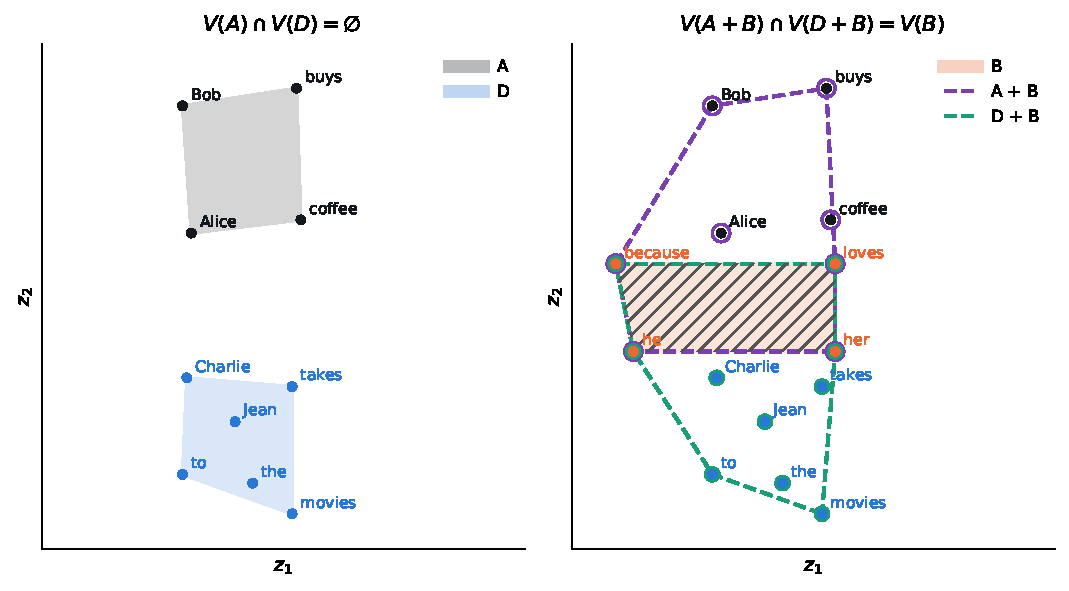
\includegraphics[width=\linewidth,height=0.8\textheight,keepaspectratio]{figures/overlap_relations_1.pdf}
\caption{Illustration, not computed from data: the first two relations on transformed points. Each dot is the point of one token in the adapted space; $z_1$ and $z_2$ are two of its dimensions. A text's volume is the smallest polygon around its tokens' points. Filled areas: texts alone. Dashed outlines and hollow circles: joined texts, whose points are the points of their parts. Hatched: the overlap of the two dashed volumes, the left side of the relation. Left: $V(A) \cap V(D) = \emptyset$; A's and D's volumes do not meet. Right: $V(A + B) \cap V(D + B) = V(B)$; A + B and D + B overlap exactly in B's volume.}
\label{fig:overlap-1}
\end{figure}

\begin{figure}[ht]
\centering
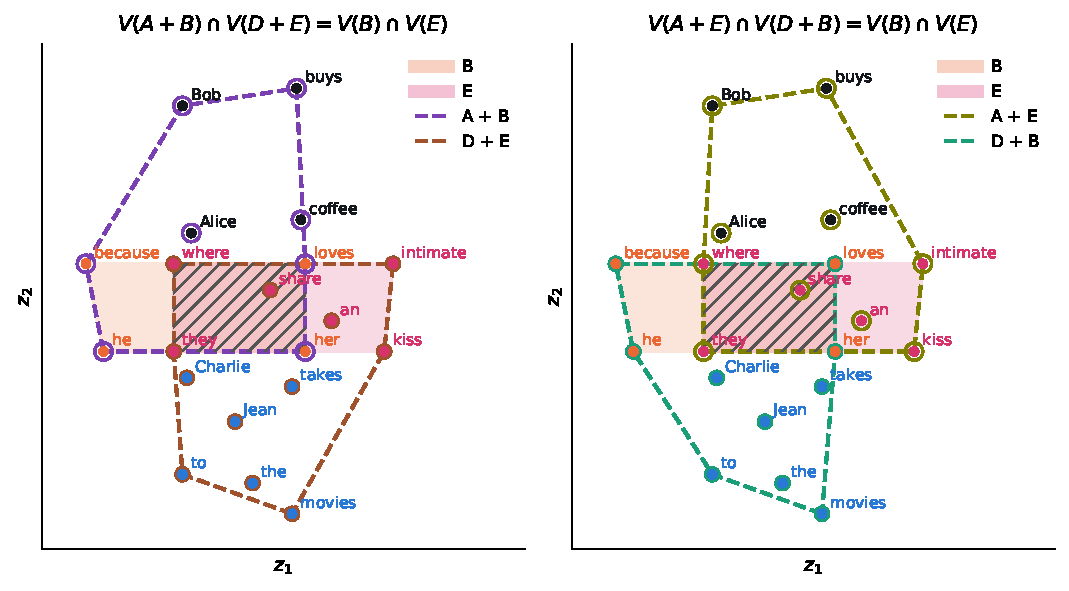
\includegraphics[width=\linewidth,height=0.8\textheight,keepaspectratio]{figures/overlap_relations_2.pdf}
\caption{Illustration, not computed from data: the last two relations on transformed points, drawn as in Figure~\ref{fig:overlap-1}. B and E overlap. Left: $V(A + B) \cap V(D + E) = V(B) \cap V(E)$; A + B and D + E overlap exactly where B and E do. Right: $V(A + E) \cap V(D + B) = V(B) \cap V(E)$; so do A + E and D + B.}
\label{fig:overlap-2}
\end{figure}

\FloatBarrier
\subsection{Alternatives we considered}\label{sec:alternatives}

\subsubsection{A deterministic transformation}

Could the transformation be computed without learning anything? No. The only deterministic, untrained signal we know of is how much a span moves Qwen's points for the text that follows it. To test it, we put a span after A and a follow-up sentence after the span, and measured how far the follow-up's points move compared with A followed directly by the same follow-up: $1$ minus the mean cosine between the two sets of points, averaged over five follow-ups (``Alice smiled.'', ``She thanked him.'', ``Then they sat down.'', ``Alice looked at him.'', ``She took a sip.'').

\begin{center}
\begin{tabular}{llc}
\hline
 & span after A & $1 - \cos$ after layer $16$ \\
\hline
motives & ``, because he loves her'' & $0.14$ \\
 & ``, since he misses her'' & $0.14$ \\
 & ``, hoping to win her'' & $0.21$ \\
\hline
details & ``and bagels with salmon'' & $0.09$ \\
 & ``with oat milk and sugar'' & $0.07$ \\
 & ``and two glasses of water'' & $0.07$ \\
 & ``, and he pays cash'' & $0.12$ \\
 & ``, with his left hand'' & $0.14$ \\
\hline
\end{tabular}
\end{center}

The signal falls short in two ways:
\begin{enumerate}
  \item \textbf{It does not separate cleanly.} The motives move the follow-ups more than the food details do, but ``and he pays cash'' and ``with his left hand'' move them almost as much as the motives.
  \item \textbf{It gives only a size.} It does not say which directions two texts share, and Requirement~\ref{req:overlap-is-shared} needs exactly that.
\end{enumerate}
Choosing the subspace that keeps B's directions and discards C's (Section~\ref{sec:properties}) needs examples of what is salient. That is learning, even when it is done in closed form rather than by gradient descent.

\subsubsection{How to train}

Qwen does not understand which information is salient (Section~\ref{sec:movement}), so every approach learns it from our labelled texts and maps it into a new space. They differ only in where the learned part sits. Qwen provides the text understanding; the learned part learns which information is salient. An approach can be used if its learned part is trained by minimising our loss, leaves Qwen's text understanding intact, and has few enough parameters for our few labelled examples. Among those that can, what the learned part sees decides how much it can learn:
\begin{center}
\small
\begin{tabular}{@{}l c c r p{0.22\linewidth} c@{}}
\hline
approach & \shortstack{trained by\\our loss} & \shortstack{Qwen\\kept intact} & \shortstack{trained\\parameters} & \shortstack{learned\\part sees} & usable \\
\hline
LoRA adapter & yes & yes & $44$ million & every layer of Qwen & yes \\
soft prompt & yes & yes & $82$ thousand & every layer, through its vectors & yes \\
fully connected head & yes & yes & $262$ thousand & Qwen's finished points & yes \\
closed-form head & no & yes & none & Qwen's finished points & no \\
retraining all of Qwen & yes & no & $8.2$ billion & every layer of Qwen & no \\
\hline
\end{tabular}
\end{center}
The soft prompt is counted as $20$ vectors of $4096$ numbers. The closed-form head fails the first test; retraining all of Qwen fails the second and the third. The head sees only Qwen's finished points, so it can learn salience only if salience is a simple function of them, and nothing indicates that it is (the conclusion of Section~\ref{sec:movement}). LoRA works inside every layer of Qwen and has no such condition, so it comes first. The soft prompt also changes what every layer computes, through its vectors, so it comes before the head too.

Sorted from the best option to start with:
\begin{center}
\small
\begin{tabular}{@{}p{0.14\linewidth} p{0.24\linewidth} c p{0.44\linewidth}@{}}
\hline
approach & mechanism & applicable & because \\
\hline
LoRA adapter & learned changes inside Qwen's layers, then a map into the new space & yes & it changes what Qwen's layers compute, so it does not depend on Qwen already computing what salience is judged from. \\
soft prompt & learned vectors before the text steer Qwen's layers & yes & like LoRA, it changes what every layer of Qwen computes, so it does not depend on Qwen already computing what salience is judged from; but it is weaker, because it changes only what the layers read, not their weights. \\
fully connected head & a learned map from Qwen's frozen points into the new space & yes & cheaper than LoRA and leaves Qwen untouched, but works only if salience is a simple function of Qwen's finished points, which nothing indicates (the conclusion of Section~\ref{sec:movement}). \\
closed-form head & a map computed by a formula from labelled texts & no & a formula, such as a difference of means, cannot be fitted to the overlap relations; only minimising a loss can \\
retraining all of Qwen & all of Qwen's weights learned anew & no & our few labelled examples cannot constrain $8.2$ billion parameters: it would overfit them and erase Qwen's knowledge of language, and costs about $130$\,GB to train and a second copy of Qwen to serve \\
\hline
\end{tabular}
\end{center}

\subsubsection{To do: LoRA adapter}
\begin{enumerate}
  \item Train the adapter and a head on the labelled texts with the volume loss.
  \item Serve with the adapter switched on per request.
\end{enumerate}

\subsubsection{To do: soft prompt}
\begin{enumerate}
  \item Train the vectors and a head on the labelled texts with the volume loss.
  \item Add an endpoint that accepts vectors in place of tokens.
\end{enumerate}

\subsubsection{To do: fully connected head}
\begin{enumerate}
  \item Run every labelled text through Qwen once and store its points.
  \item Train the head on them with the volume loss.
  \item Test the relations on texts it was not trained on.
\end{enumerate}

\end{document}
